\documentclass{article}
\usepackage{graphicx} % Required for inserting images

\title{ARK}
\author{Samiya Singhal}
\date{March 2025}

\begin{document}

\maketitle

\section{Task 1}
In task 1, I first converted the images into grayscale images and then created an array of these images.  After that, I created a 2D NumPy array of the size of the array of images and assigned the value 0 to all the elements. Then assuming that the maximum shift is 64 pixels, I have calculated the best shift for every element of the array.  The values were then scaled to 0-255 from 0-64. Next, I have set the values for r, g, b according to the grayscale values of the pixels, and hence obtained the depth map.
\begin{figure}[h!]
    \centering
    \includegraphics[width=1\linewidth]{Depth map.png}
\end{figure}

The above is the picture of the depth map.

\section{Task 2}
First, I have converted pi image into a grayscale image and then into a numpy array. Next as the distorted pixels are white they have the highest grayscale value and hence when the whole array is divided by 10 * pi, the value of the distorted pixels is going to be the greatest. Thus the 2x2 filter constitutes of the 4 corrected pixels' values.  Next I have created a function which takes an image, filter matrix and operation as an input and returns the original image after applying the filter to the distorted image. After applying the function and restoring the original potrait, I have scaled it up to size (100, 100). Next I have created a function for template matching and hence obtained the x and y coordinates as (659, 32) and the password as 2170.

The following is the picture of the restored potrait scaled up to dimension 100x100.
\begin{figure}[h!]
    \centering
    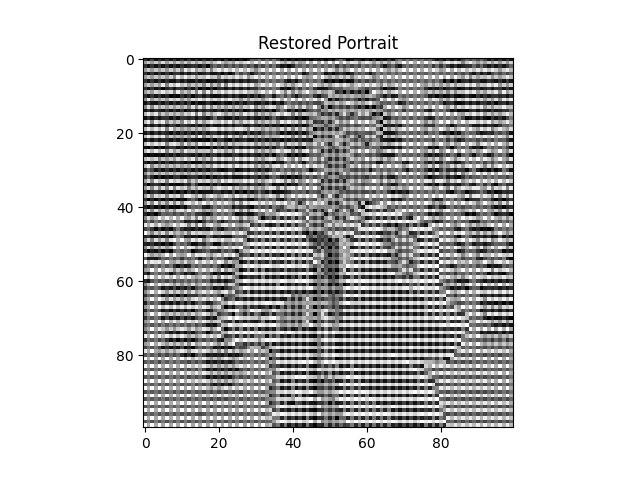
\includegraphics[width=1\linewidth]{Restored potrait.png}
\end{figure}

\section{Task 3}
In this I first converted the image maze into a graysacale image. The image is then converted into a binary format to make path computation easier. Next, the algorithm randomly takes sample points in the free space, ensuring that they do not overlap with obstacles. These points serve as potential waypoints for constructing a roadmap.

To connect these waypoints, the algorithm uses a k-nearest neighbors (k-NN) approach, identifying the closest points and checking if a direct path between them is collision-free. A collision-checking function ensures that no point along the straight-line path between two waypoints intersects with an obstacle. If the path is clear, an edge is added to the roadmap graph, with the distance between waypoints as the edge weight.

Once the roadmap is built, Dijkstra’s algorithm is applied to find the shortest path between the given start and goal locations. If a valid path exists, the roadmap and final path are visualized using OpenCV, where the roadmap is displayed in gray and the final path is marked in red. To further illustrate the movement, a Pygame-based simulation animates the robot as it follows the computed path through the maze.
Following is the image of the path that I got. I couldn't improve much on the algorithm due to time constraint.
\begin{figure}[h!]
    \centering
    \includegraphics[width=0.5\linewidth]{path.png}
\end{figure}

 
\end{document}
